\documentclass[9pt,technote]{IEEEtran}
\usepackage{amsmath,amssymb,amsfonts}
\usepackage{algorithmic}
\usepackage{graphicx}
\usepackage{textcomp}
\usepackage{xcolor}
\usepackage{listings}
\usepackage{booktabs}
\usepackage{array}
\usepackage{hyperref}
\usepackage{siunitx}
\usepackage{float}

\begin{document}

\title{ATLAS: Autonomous Traffic Light And Sign System\\
\Large A ROS2-based Implementation for Automated Navigation}

\author{Alberto Finardi, Federico Romano, Francesco De Vito}
\maketitle

\begin{abstract}
This paper presents ATLAS (Autonomous Traffic Light And Sign System), a comprehensive ROS2-based solution for autonomous robot navigation with traffic sign and signal recognition capabilities. The system implements robust line-following using computer vision and PID control, along with traffic element recognition using ArUco markers. We detail the architecture, explain the communication between distributed nodes, and analyze parameter sensitivity. Our implementation demonstrates the integration of perception, decision-making, and control for autonomous navigation in structured environments. The experimental results validate the system's ability to follow paths reliably while recognizing and responding appropriately to traffic signs and signals, providing a foundation for more complex autonomous navigation applications.
\end{abstract}

\section{Introduction}
Autonomous vehicles must accurately perceive and respond to environmental elements including lane markings, traffic signs, and signals. The ATLAS project addresses these challenges through a scaled-down simulation implemented on a mobile robot platform. Using a RoboMaster S1 equipped with cameras and sensors, the system demonstrates fundamental capabilities required for autonomous navigation: path following using computer vision and PID control, traffic light and sign recognition, and decision-making and motion control.

Unlike many existing implementations, ATLAS integrates perception, decision-making, and control into a cohesive system. The distributed ROS2 architecture allows for modularity, extensibility, and robust performance. A key design choice was to rely exclusively on computer vision and velocity commands, deliberately avoiding other sensors or odometry to make the robot "less aware" of its internal state and more responsive to the external environment.

The project provides default models for the Robomaster S1 robot with additional vision sensors and traffic light cubes (under \texttt{models} and \texttt{scenes} in the root folder). The traffic light cubes must be used carefully as their orientation is critical - if rotated incorrectly, the faces of the cube are misaligned and may not be recognized properly. Additionally, the project includes a complete test scene containing a circuit with all the traffic signs and turns designed to validate the system's functionality under various conditions.

It is also easily adaptable to the RoboMaster EP by using an appropriate model with the additional vision sensors for line-following functionality and updating the launch files to use the correct drivers. Moreover, since the system relies solely on computer vision and velocity commands, it can theoretically be deployed on any four-wheeled robot with compatible hardware and software interfaces.

\section{Background}
Autonomous navigation has been extensively studied in the robotics and computer vision communities. Path following using vision-based approaches has evolved from simple line detection techniques to more sophisticated deep learning methods. Traffic sign recognition has similarly progressed from template matching to convolutional neural networks.

In the educational context, smaller platforms like Duckietown provide environments for teaching autonomous navigation concepts. ATLAS builds upon these approaches while emphasizing the integration of multiple perception and control modules within the ROS2 framework.

\section{System Architecture}
ATLAS is built on ROS2, leveraging its distributed architecture and publish-subscribe communication model. The system consists of three primary nodes:

\begin{itemize}
    \item \textbf{Line PID Node}: Processes camera images to detect lines and calculate appropriate steering commands
    \item \textbf{Traffic Detection Node}: Analyzes camera input to recognize traffic signs and signals
    \item \textbf{Controller Node}: Integrates information from the other nodes to control the robot's movement
\end{itemize}

Fig. \ref{fig:system_architecture} illustrates the system architecture and communication flow between nodes.

\begin{figure}[H]
    \centering
    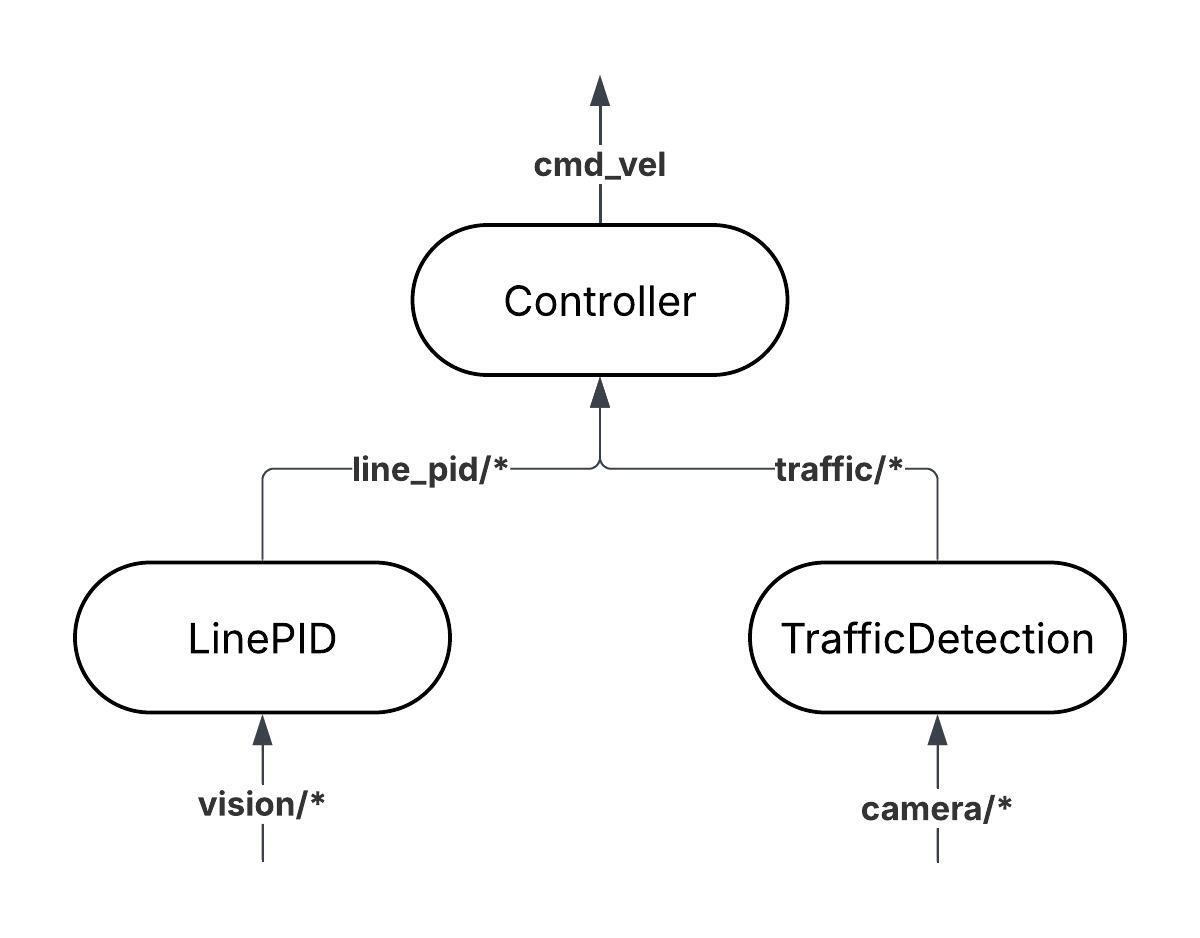
\includegraphics[width=0.6\columnwidth]{figures/architecture.jpeg}
    \caption{ROS2 node graph showing the communication flow between the three primary nodes of the ATLAS system and their interactions with the robot's sensors and actuators.}
    \label{fig:system_architecture}
\end{figure}

\subsection{System Deployment and Launch Configuration}
The entire ATLAS system is deployed through a centralized ROS2 launch file, which configures all nodes and their parameters in a unified manner. This approach ensures consistent initialization and proper integration between components. Within the launch file, all topic names are specified with namespaces relative to the robot's name, allowing for potential multi-robot deployments with minimal configuration changes.

A debug launch file is also provided, which includes additional visualization tools for monitoring the system's performance. This debug configuration can be used to visualize the cameras feed after image processing and/or with information overlay.

The vision system for the robot (\texttt{/vision/left}, \texttt{/vision/center}, \texttt{/vision/right}) is implemented directly in the Coppelia simulation environment using a Lua script. This script simulates the robot's cameras and publishes the visual data to the ROS2 network, where it's consumed by the Line PID Node. 

It's important to note that while other topics use relative paths beginning with the robot name, the vision sensor topics created by the Lua scripts use absolute paths. This means that for multi-robot simulations, both the Lua scripts and the Line PID Node would need to be modified to ensure the correct topic mapping. The Lua scripts would need to generate unique topic names per robot, and the Line PID Node would need to subscribe to the correct robot-specific vision topics rather than the current absolute ones.

\subsection{Code Structure and Organization}
The ATLAS system is organized into three Python modules, each implementing one of the primary nodes. The structure follows ROS2 best practices with clear separation of concerns:

\begin{itemize}
    \item \texttt{line\_pid\_node.py}: Implements the \texttt{LinePIDNode} class that handles line detection and PID-based steering
    \item \texttt{traffic\_detection\_node.py}: Implements the \texttt{TrafficDetectorNode} class for ArUco marker recognition
    \item \texttt{controller\_node.py}: Implements the \texttt{ControllerNode} class that handles decision-making and motion control
\end{itemize}

Each module follows a consistent pattern with class definitions, ROS2 publisher/subscriber initialization, parameter declaration, callback methods for handling sensor inputs, and helper methods for processing data and controlling outputs.

\subsection{Communication Paradigm}
The nodes communicate through ROS2 topics using standard message types. The key topics include:

\begin{itemize}
    \item \texttt{/vision/left}, \texttt{/vision/center}, \texttt{/vision/right}: Camera feeds for line detection
    \item \texttt{camera/image\_color}: Camera feed for traffic sign detection
    \item \texttt{line\_pid/steering}: Normalized steering values from the PID controller [-1.0 to +1.0]
    \item \texttt{line\_pid/stop\_line\_detected}: Boolean indicating stop line detection
    \item \texttt{line\_pid/lost\_line\_detected}: Boolean indicating lost line detection
    \item \texttt{traffic/id}: Detected traffic sign/light identifier
    \item \texttt{cmd\_vel}: Velocity commands for the robot
\end{itemize}

Additional topics are available launching the debug configuration, including:
\begin{itemize}
    \item \texttt{line\_pid/debug/left\_cam}: Debug camera feed from the left line-following camera (post-processed)
    \item \texttt{line\_pid/debug/center\_cam}: Debug camera feed from the center line-following camera (post-processed)
    \item \texttt{line\_pid/debug/right\_cam}: Debug camera feed from the right line-following camera (post-processed)
    \item \texttt{traffic/debug/overlay}: Debug camera feed from the Traffic Detection Node, overlaying the detected ArUco markers on the original image
    \item \texttt{traffic/debug/processed}: Debug camera feed from the Traffic Detection Node, overlaying the detected ArUco markers on the processed image
\end{itemize}


\subsection{Parameter Management}
Each node exposes configurable parameters through the ROS2 parameter system, allowing for adjustment of behavior. This design choice enables fine-tuning of the system without code modification and supports adaptation to different environmental conditions.

\section{Line PID Node Implementation}
The Line PID Node is responsible for processing camera images to detect lines and calculate steering commands using a proportional-integral-derivative (PID) control approach.

\subsection{Multi-Camera Line Detection}
The system employs three cameras positioned to provide comprehensive path visibility. A deliberate design choice was made to use three low-resolution cameras (16×16 pixels) rather than a single high-resolution camera. This approach more accurately represents real-world robotic scenarios where processing constraints and sensor limitations are common, and it provides inherent redundancy and wider spatial awareness.

Each camera's image is processed independently through an image processing pipeline:

\begin{enumerate}
    \item \textbf{Image Pre-processing:} The raw RGB image is converted to BGR if needed, resized to 16×16 resolution, and rotated 90 degrees counterclockwise.
    
    \item \textbf{Grayscale Conversion and Blur:} The image is converted to grayscale and a Gaussian blur is applied to reduce noise.
    
    \item \textbf{Binary Thresholding:} The blurred image is converted to a binary image using an inverted threshold.
    
    \item \textbf{Contour Detection:} OpenCV's contour detection algorithm identifies continuous shapes in the binary image.
    
    \item \textbf{Contour Analysis:} The largest contour is selected as the most likely candidate for the line if its area exceeds the minimum threshold.
    
    \item \textbf{Position Normalization:} The horizontal position of the line is normalized to a range of 0.0 to 1.0 using the moments of the contour.
\end{enumerate}

\begin{figure}[H]
 \centering
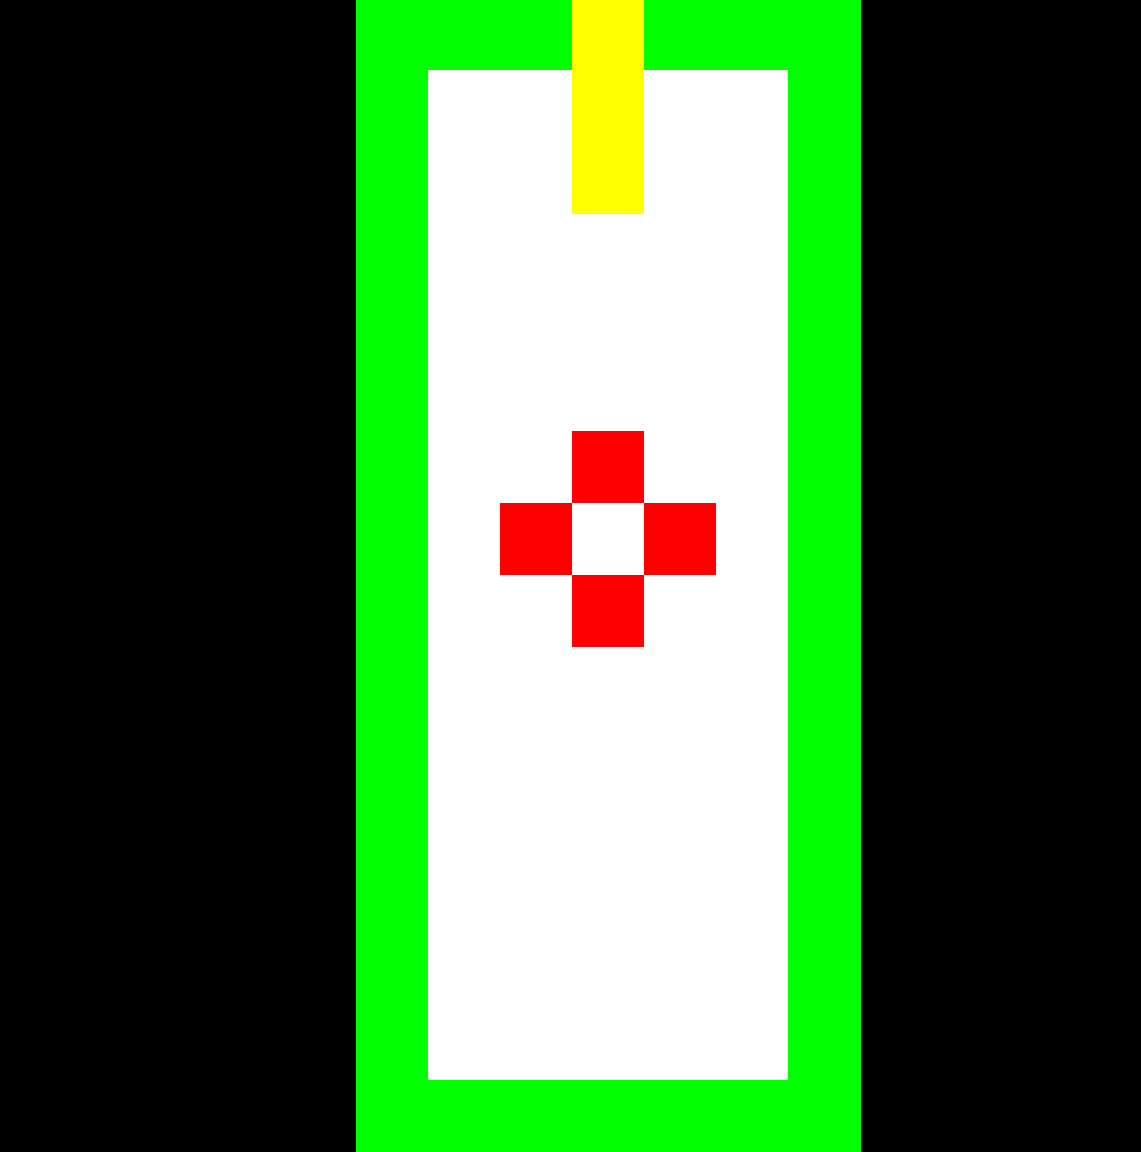
\includegraphics[width=0.6\columnwidth]{figures/line_detection_cameras.png}
\caption{Debug visualization from the line detection system. The white area represents the binary-thresholded image where the path line has been detected. The green borders show the edge of the track visible to the camera. The line position is shown with a yellow line. The red cross pattern highlights the centroid marker of the detected contour, showing the calculated center point of the line for PID control purposes.}
\label{fig:camera_debug}
\end{figure}

The normalized positions have different target values based on camera position:
\begin{itemize}
    \item Left camera: Target position 0.0 (left edge)
    \item Center camera: Target position 0.5 (center)
    \item Right camera: Target position 1.0 (right edge)
\end{itemize}

\subsection{PID Control Implementation}
Each camera has an independent PID controller with tunable parameters that can be adjusted through the ROS2 parameter system. The control system uses different proportional, integral, and derivative gains for each camera to account for their different perspectives.

The PID control implementation involves:

\begin{enumerate}
    \item \textbf{Error Calculation:} The error is calculated as the difference between the detected line position and the target position for each camera.
    
    \item \textbf{PID Term Calculation:} For each camera's error value, the system calculates proportional, integral, and derivative terms.
    
    \item \textbf{Integral Anti-windup:} The accumulated integral value is clamped to configurable limits to prevent excessive overshoot.
    
    \item \textbf{Derivative Filtering:} A moving average filter is applied to the derivative term to reduce sensitivity to noise.
    
    \item \textbf{Sharp Turn Detection:} The system automatically detects sharp turns by analyzing discrepancies between camera readings and adjusts control parameters accordingly.
    
    \item \textbf{Weighted Output Fusion:} The PID outputs from each camera are combined using a weighted average based on proportional gain parameters.
    
    \item \textbf{Output Normalization:} The final steering command is normalized to a range of -1.0 to +1.0 using a hyperbolic tangent function.
\end{enumerate}

\subsection{Stop Line Detection}
The system detects stop lines by analyzing positions from all three cameras simultaneously, looking for:

\begin{itemize}
    \item \textbf{Multi-camera Confirmation:} Detection in all three cameras simultaneously
    \item \textbf{Position Consistency:} Line positions across all cameras within a configurable deviation threshold
    \item \textbf{Centered Detection:} Average position near the center of the field of view
\end{itemize}

\subsection{Lost Line Detection}
If no lines are detected across all cameras for a sustained period (configurable timeout parameter), the system signals a lost line condition, ensuring safe behavior when the robot encounters gaps or moves out of the designated route. This temporal threshold is crucial as it prevents false triggers from momentary detection failures, while still ensuring timely response to actual line loss situations.

\subsection{Parameters Analysis}
The Line PID Node's behavior can be significantly altered by adjusting its parameters (Table \ref{tab:pid_params}).

\begin{table}[H]
\centering
\caption{Line PID Node Parameters and Their Impact}
\label{tab:pid_params}
\begin{tabular}{@{}p{0.3\columnwidth}p{0.11\columnwidth}p{0.5\columnwidth}@{}}
\toprule
\textbf{Parameter} & \textbf{Default} & \textbf{Impact of Changes} \\
\midrule
\parbox[t]{0.30\columnwidth}{\texttt{threshold\textunderscore}\texttt{value}} & 128 & Higher values increase sensitivity to bright lines, lower values to darker lines \\
\midrule
\parbox[t]{0.30\columnwidth}{\texttt{min\textunderscore}\texttt{contour\textunderscore}\\\texttt{area}} & 3 & Lower values increase sensitivity but may introduce noise \\
\midrule
\parbox[t]{0.30\columnwidth}{\texttt{debug}} & False & Enable debug camera feeds \\
\midrule
\parbox[t]{0.30\columnwidth}{\texttt{stop\textunderscore}\texttt{line\textunderscore}\texttt{max\textunderscore}\\\texttt{deviation}} & 0.15 & Higher values allow more positional variation between cameras for stop line detection, but may cause false positives \\
\midrule
\parbox[t]{0.30\columnwidth}{\texttt{stop\textunderscore}\texttt{line\textunderscore}\texttt{center\textunderscore}\\\texttt{min}} & 0.4 & Lower values detect stop lines earlier (when they first appear at the bottom of the image) \\
\midrule
\parbox[t]{0.30\columnwidth}{\texttt{stop\textunderscore}\texttt{line\textunderscore}\texttt{center\textunderscore}\\\texttt{max}} & 0.6 & Higher values detect stop lines later (when they're closer to the center of the image) \\
\midrule
\parbox[t]{0.30\columnwidth}{\texttt{*\textunderscore kp}} & 0.8-1.0 & Higher proportional gain increases responsiveness but may cause oscillation \\
\midrule
\parbox[t]{0.30\columnwidth}{\texttt{*\textunderscore ki}} & 0.02 & Higher integral gain improves steady-state error but may cause overshoot \\
\midrule
\parbox[t]{0.30\columnwidth}{\texttt{*\textunderscore kd}} & 0.35-0.4 & Higher derivative gain reduces overshoot but may amplify noise \\
\midrule
\parbox[t]{0.30\columnwidth}{\texttt{integral\textunderscore}\texttt{windup\textunderscore}\\\texttt{limit}} & 0.2 & Lower values reduce potential overshoot but limit error correction \\
\midrule
\parbox[t]{0.30\columnwidth}{\texttt{corner\textunderscore}\texttt{detection\textunderscore}\\\texttt{threshold}} & 0.25 & Lower values make corner detection more sensitive \\
\bottomrule
\end{tabular}
\end{table}

\section{Traffic Detection Node Implementation}
The Traffic Detection Node processes camera images to recognize traffic signs and signals using ArUco markers as fiducial references.

\subsection{ArUco Marker Detection Logic}
ArUco markers are square fiducial markers with a black background and an internal binary pattern that uniquely identifies each marker. The detection algorithm involves:

\begin{enumerate}
    \item \textbf{Image Pre-processing:} The input image is converted to grayscale and processed with a Gaussian blur to reduce noise.
    
    \item \textbf{Multi-threshold Approach:} Rather than using a single threshold value, which might fail under varying lighting conditions, the system applies multiple thresholds between configurable minimum and maximum values. This adaptive approach significantly improves detection reliability across different lighting scenarios.
    
    \item \textbf{Contour Analysis:} For each detected marker, the system calculates the contour perimeter as a measure of marker size and the center position.
    
    \item \textbf{Marker Filtering:} A filtering process selects the instance with the largest perimeter if multiple markers are detected.
\end{enumerate}

\begin{figure}[H]
    \centering
    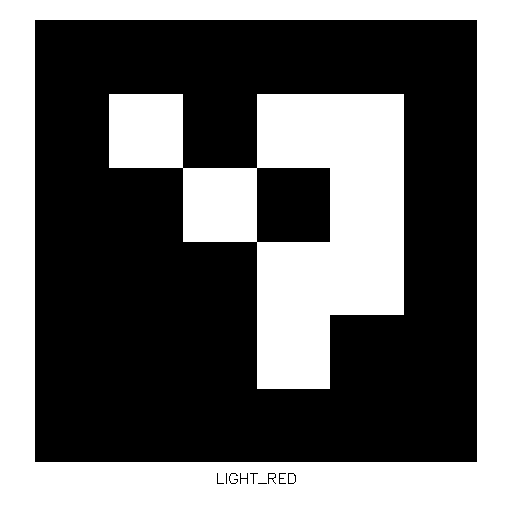
\includegraphics[width=0.6\columnwidth]{figures/aruco_markers_placeholder.png}
    \caption{Example ArUco markers used for traffic sign recognition, showing the distinctive patterns for different traffic elements.}
    \label{fig:aruco_markers}
\end{figure}

\subsection{Traffic Element Mapping}
The system maps ArUco marker IDs to specific traffic elements:

\begin{itemize}
    \item ID 0: Red traffic light
    \item ID 1: Yellow traffic light
    \item ID 2: Green traffic light
    \item ID 3: Speed limit 30 km/h
    \item ID 4: Speed limit 50 km/h
\end{itemize}

\subsection{Detection Confidence Tracking}
To improve reliability, the node implements a confidence tracking system:

\begin{itemize}
    \item \textbf{Consistency Counting:} A confidence counter is incremented when the same marker ID is detected in consecutive frames.
    
    \item \textbf{Reset on Change:} The confidence counter is reset to 1 when a different marker ID is detected.
    
    \item \textbf{Confidence Threshold:} A detection is only considered valid when the confidence counter exceeds a configurable threshold.
    
    \item \textbf{Gradual Confidence Decay:} The confidence counter is decremented rather than immediately reset when no markers are detected.
\end{itemize}

\subsection{Parameters Analysis}
The Traffic Detection Node's behavior can be adjusted through several parameters (Table \ref{tab:traffic_params}).

\begin{table}[H]
\centering
\caption{Traffic Detection Node Parameters and Their Impact}
\label{tab:traffic_params}
\begin{tabular}{@{}p{0.3\columnwidth}p{0.1\columnwidth}p{0.5\columnwidth}@{}}
\toprule
\textbf{Parameter} & \textbf{Default} & \textbf{Impact of Changes} \\
\midrule
\parbox[t]{0.30\columnwidth}{\texttt{min\textunderscore}\texttt{threshold}} & 40 & Lower values detect darker markers but may increase false positives \\[2ex]
\midrule
\parbox[t]{0.30\columnwidth}{\texttt{max\textunderscore}\texttt{threshold}} & 150 & Higher values detect lighter markers but may miss darker ones \\[2ex]
\midrule
\parbox[t]{0.30\columnwidth}{\texttt{threshold\textunderscore}\texttt{step}} & 20 & Smaller steps improve detection at the cost of processing time \\[2ex]
\midrule
\parbox[t]{0.30\columnwidth}{\texttt{min\textunderscore}\texttt{detection\textunderscore}\\\texttt{confidence}} & 10 & Higher values reduce false positives but increase detection delay \\
\bottomrule
\end{tabular}
\end{table}

\section{Controller Node Implementation}
The Controller Node integrates information from the Line PID Node and Traffic Detection Node to generate appropriate motion commands for the robot.

\subsection{State Management Logic}
The Controller Node maintains internal state information critical for decision-making:

\begin{itemize}
    \item \textbf{Traffic Light State:} Boolean flags for red or yellow light detection
    \item \textbf{Line Detection State:} Tracking of stop lines or lost lines
    \item \textbf{Velocity State:} Current linear and angular velocities, including a "green light" reference velocity
    \item \textbf{Operation State:} Tracking of startup delay, running, or stopped modes
\end{itemize}

\subsection{Motion Control Architecture}
The Controller Node serves as the central integration point for the ATLAS system, subscribing to:

\begin{itemize}
    \item \textbf{Steering Commands (\texttt{line\_pid/steering}):} Normalized steering values (-1.0 to +1.0)
    \item \textbf{Stop Line Detection (\texttt{line\_pid/stop\_line\_detected}):} Boolean signals for stop lines
    \item \textbf{Traffic Sign Information (\texttt{traffic/id}):} Identifiers for detected traffic signs and signals
\end{itemize}

The motion control loop runs at 30Hz, calculating appropriate linear and angular velocities and publishing velocity commands to the robot's \texttt{cmd\_vel} topic.

\subsection{Traffic Sign Integration}
The Controller Node implements a state machine approach to integrate traffic sign information into navigation behavior:

\begin{itemize}
    \item \textbf{Traffic Lights:}
    \begin{itemize}
        \item Red Light: Reduces speed and sets the "red light detected" flag
        \item Yellow Light: Reduces speed and sets the "yellow light detected" flag
        \item Green Light: Resumes movement at the previously set "green light" velocity
    \end{itemize}
    
    \item \textbf{Speed Limits:}
    \begin{itemize}
        \item Speed 30: Sets the linear velocity to a slower value
        \item Speed 50: Sets the linear velocity to a faster value
    \end{itemize}
\end{itemize}

\subsection{Safety Features}
The Controller Node implements several safety mechanisms:

\begin{itemize}
    \item \textbf{Startup Delay:} A configurable delay before allowing movement
    \item \textbf{Lost Line Response:} Immediate stop when the line is lost
    \item \textbf{Stop Line Response:} Appropriate action based on traffic light state
    \item \textbf{Emergency Stop:} A dedicated method to halt movement when required (i.e. stop line and red light, or lost line)
    \item \textbf{Incorrect slowing down:} A configurable timeout is set to prevent unwanted slowdowns when traffic lights remain visible after the vehicle has passed through a stop line, thus ignoring the traffic light if still in field of view.
\end{itemize}

\subsection{Parameters Analysis}
The Controller Node's parameters significantly affect the robot's behavior (Table \ref{tab:controller_params}).

\begin{table}[H]
\centering
\caption{Controller Node Parameters and Their Impact}
\label{tab:controller_params}
\begin{tabular}{@{}p{0.3\columnwidth}p{0.1\columnwidth}p{0.5\columnwidth}@{}}
\toprule
\textbf{Parameter} & \textbf{Default} & \textbf{Impact of Changes} \\
\midrule
\parbox[t]{0.30\columnwidth}{\texttt{linear\textunderscore}\texttt{velocity\textunderscore\\50}} & 1.0 & Higher values increase maximum speed but may reduce control precision \\[2ex]
\midrule
\parbox[t]{0.30\columnwidth}{\texttt{linear\textunderscore}\texttt{velocity\textunderscore\\30}} & 0.5 & Higher values increase reduced speed mode but may compromise safety in constrained areas \\[2ex]
\midrule
\parbox[t]{0.30\columnwidth}{\texttt{angular\textunderscore}\texttt{velocity\textunderscore}\\\texttt{max}} & 2.0 & Higher values enable sharper turns but may cause instability \\[2ex]
\midrule
\parbox[t]{0.30\columnwidth}{\texttt{startup\textunderscore}\texttt{delay}} & 5.0 & Longer delay ensures stable initialization but increases wait time \\[2ex]
\midrule
\parbox[t]{0.30\columnwidth}{\texttt{stop\textunderscore}\texttt{line\textunderscore}\texttt{timeout}} & 2.0 & Prevents unwanted slowdowns when traffic lights remain visible after the vehicle has passed through a stop line  \\
\bottomrule
\end{tabular}
\end{table}

\section{Experimental Results}
The ATLAS system was tested in a controlled environment with a predefined path and various traffic elements, demonstrating line following, navigation, stop line detection, traffic light recognition, and speed adjustment.

\subsection{Line Following Performance}
The line following system demonstrated robust performance with the following observations:

\begin{itemize}
    \item \textbf{Speed-Accuracy Trade-off:} Lower speeds provided the most accurate line following with maximum turn angles.
    \item \textbf{Multi-Camera Advantage:} The multi-camera approach improved performance on curves.
    \item \textbf{Lighting Sensitivity:} Performance remained consistent under moderate lighting variations.
    \item \textbf{Recovery Capabilities:} The system successfully recovered from temporary line loss conditions.
\end{itemize}

\subsection{Traffic Recognition Performance}
The traffic sign recognition system showed the following characteristics:

\begin{itemize}
    \item \textbf{Detection Range:} Optimal detection occurred at lower distances from the camera.
    \item \textbf{False Positive Elimination:} The confidence tracking system effectively eliminated false positives.
    \item \textbf{Lighting Adaptation:} The multi-threshold approach significantly improved detection under varying lighting conditions.
    \item \textbf{Processing Efficiency:} The system maintained sufficient responsiveness for real-time operation.
\end{itemize}

\subsection{Integrated System Performance}
Tests of the complete integrated system revealed:

\begin{itemize}
    \item \textbf{Navigation Accuracy:} Successful navigation with low path deviation.
    \item \textbf{Traffic Rule Compliance:} Appropriate responses to all traffic elements.
    \item \textbf{Continuous Operation:} Consistent performance during extended testing.
\end{itemize}

\subsection{Edge Cases and Robustness Analysis}
The system successfully handled edge cases including simultaneous traffic signs, rapid traffic light changes, line interruptions, and sharp turns.

\section{Discussion}

\subsection{Integration of Multiple Perception Sources}
The combination of line detection and marker detection creates a more robust navigation system than either approach alone. The multi-camera approach provided redundancy and broader spatial awareness, while the weighted fusion of camera inputs created a system that could smoothly transition between different perceptual regimes without explicit mode switching.

The deliberate choice to rely exclusively on computer vision and velocity commands, without using odometry or additional sensors, proved to be a significant advantage for environmental adaptability. By making the robot "less aware" of its internal state, the system was forced to continuously react to its environment rather than depending on potentially error-prone self-localization.

\subsection{Parameter Tuning Trade-offs}
Throughout development, we observed several trade-offs in parameter configuration:

\begin{itemize}
    \item \textbf{Control Responsiveness vs. Stability:} Higher PID gains improved responsiveness but increased oscillation risk.
    \item \textbf{Speed vs. Accuracy:} Faster speeds improved efficiency but reduced detection reliability and control precision.
    \item \textbf{Detection Confidence vs. Latency:} Higher confidence thresholds reduced false positives but increased detection latency.
    \item \textbf{Image Processing Complexity vs. Computational requirements:} More sophisticated techniques improved detection but required additional computational resources.
\end{itemize}

\subsection{Modular Design Benefits}
The separation of perception, decision-making, and control into different nodes provided several advantages:

\begin{itemize}
    \item \textbf{Isolated Testing:} Each component could be tested independently.
    \item \textbf{Reconfigurability:} Different configurations could be evaluated without modifying the controller node.
    \item \textbf{Failure Isolation:} Issues in one component did not necessarily compromise the entire system.
\end{itemize}

\subsection{Simulation to Reality Transfer Challenges}
For real-world deployment, several considerations were identified:

\begin{itemize}
    \item \textbf{Lighting Variability:} Real-world lighting conditions are significantly more variable than simulation.
    \item \textbf{Processing Latency:} Real-world deployments might face increased processing latency due to hardware constraints.
    \item \textbf{Environmental Noise:} Physical environments introduce various noise sources not present in simulation.
\end{itemize}

\section{Conclusion}
The ATLAS project successfully delivered a comprehensive ROS2-based solution for autonomous navigation with traffic sign and signal recognition. The system integrates line following capabilities with traffic element detection to create a unified navigation solution that follows paths and obeys traffic rules.

\subsection{Possible Extensions}
The modular architecture provides a foundation that could be extended in several ways:

\begin{itemize}
    \item \textbf{Advanced Traffic Recognition:} Replacing ArUco markers with a CNN-based traffic sign recognition system.
    \item \textbf{Dynamic Obstacle Avoidance:} Integrating LIDAR or stereo vision systems for obstacle detection.
    \item \textbf{Path Planning:} Adding high-level path planning capabilities for complex environments.
    \item \textbf{Resource Optimization:} Optimizing algorithms for deployment on resource-constrained platforms.
\end{itemize}

The current implementation, complete with the Robomaster S1 model with custom vision sensors, ArUco-based traffic signs, and test circuit, provides a great foundation for extension of this autonomous navigation systems. The included test scene allows for comprehensive validation of all system components under controlled conditions, while the modular architecture enables incremental improvements and extensions without requiring a complete redesign.

\end{document}